%\UseRawInputEncoding
\documentclass{article}
\setcounter{secnumdepth}{0}
\usepackage[T1]{fontenc}
\usepackage[utf8]{inputenc}
%\usepackage[latin1]{inputenc}
%\usepackage[english, norsk]{babel}
\usepackage{filecontents}
\usepackage{tcolorbox}
\usepackage{url}
\usepackage{etoolbox}
\usepackage{framed}
\usepackage{framed, color}
\usepackage{xcolor}
\usepackage{mdframed}
\usepackage{float}
\usepackage{gensymb}
\usepackage{amsmath}

\definecolor{Black}{rgb}{0.0, 0.0, 0.0}

%Definer kode
\usepackage{listings}
\usepackage{color}
\definecolor{dkgreen}{rgb}{0,0.6,0}
\definecolor{gray}{rgb}{0.5,0.5,0.5}
\definecolor{mauve}{rgb}{0.58,0,0.82}

\lstset{frame=tb,
extendedchars = true,
texcl=true,
  language=C++,
  aboveskip=3mm,
  belowskip=3mm,
  showstringspaces=false,
  columns=flexible,
  basicstyle={\small\ttfamily},
  numbers=none,
  numberstyle=\tiny\color{gray},
  keywordstyle=\color{blue},
  commentstyle=\color{dkgreen},
  stringstyle=\color{mauve},
  breaklines=true,
  breakatwhitespace=true,
  tabsize=3
}

\usepackage[colorlinks]{hyperref}
\hypersetup{citecolor=Black}
\hypersetup{linkcolor=Black}
\hypersetup{urlcolor=Black}
\usepackage{cleveref}


\setlength{\parindent}{0em}
\setlength{\parskip}{1em}
%\renewcommand{\baselinestretch}{2.0}

%\renewcommand\thesubsection{\alph{subsection}}

\renewcommand{\figurename}{Figure}
\begin{document}
\author{Kent Odde}
\title{Assignment 2 \\DCS3101}

\maketitle
\thispagestyle{empty}
\begin{center}
\includegraphics[width=\linewidth,height=0.2\textheight,keepaspectratio]{img/USN.png}
\end{center}
\newpage

\tableofcontents

\newpage

\section{Abstract}

This is the submission for the second assignment in the course DCS-3101, Introduction to Cybersecurity, at USN Kongsberg, fall of 2020.

%Innholdsfortegnelse
\section{Q1}

There are several ways of displaying an algorithm, I have chosen to include a visual representation first:
\begin{figure}[H]
 \centering
  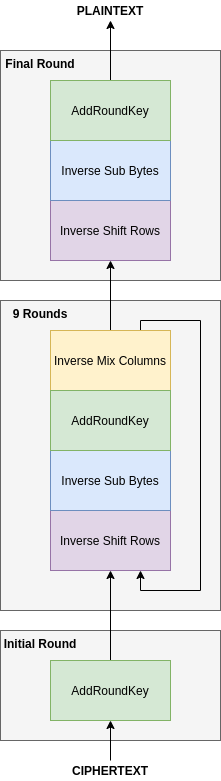
\includegraphics[width=100pt]{img/decryptAES.png}
 \caption{Algorithm for decrypting AES}
 \end{figure}


However, as code is perhaps the most precise way to describe an algorithm, and I already happen to have implemented AES encryption in C++, i decided to also include the decrypt function from that implementation: 

\begin{lstlisting}
std::string AES::decrypt128BitMessage(std::string cipherText, std::string keyString)
{
	auto key = generateGridFromHexString(keyString);
	auto grid = generateGridFromHexString(cipherText);
	auto expandedKey = generateExpandedKey(key);

	//Initial Round:
	addRoundKey(grid, expandedKey.at(expandedKey.size() - 1));

	//9 Rounds
	for(int i = expandedKey.size() - 2; i > 0; i--)
	{
		invShiftGrid(grid);
		invSubstitute(grid);
		addRoundKey(grid, expandedKey.at(i));
		invMixColumns(grid);
	}

	//Final Round
	invShiftGrid(grid);
	invSubstitute(grid);
	addRoundKey(grid, expandedKey.at(0));

	return gridToHexString(grid);
}
\end{lstlisting}

\newpage
\section{Q2}


\begin{figure}[H]
 \centering
  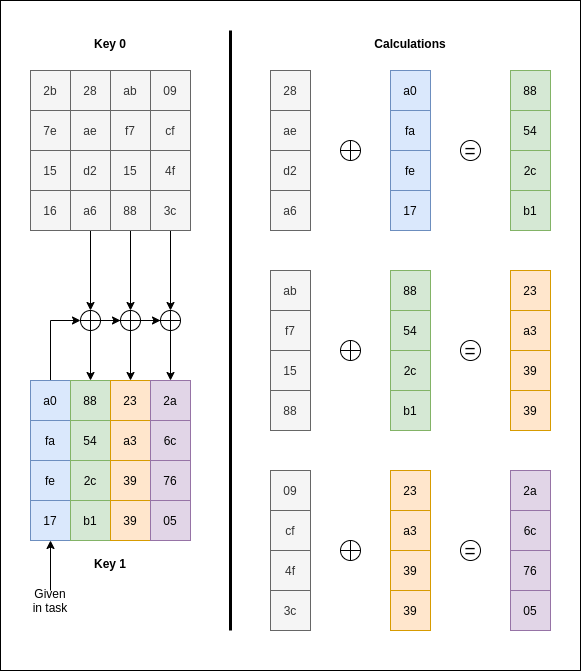
\includegraphics[width=300pt]{img/AESKey1.png}
 \caption{Calculating the first round key}
 \end{figure}

\begin{figure}[H]
 \centering
  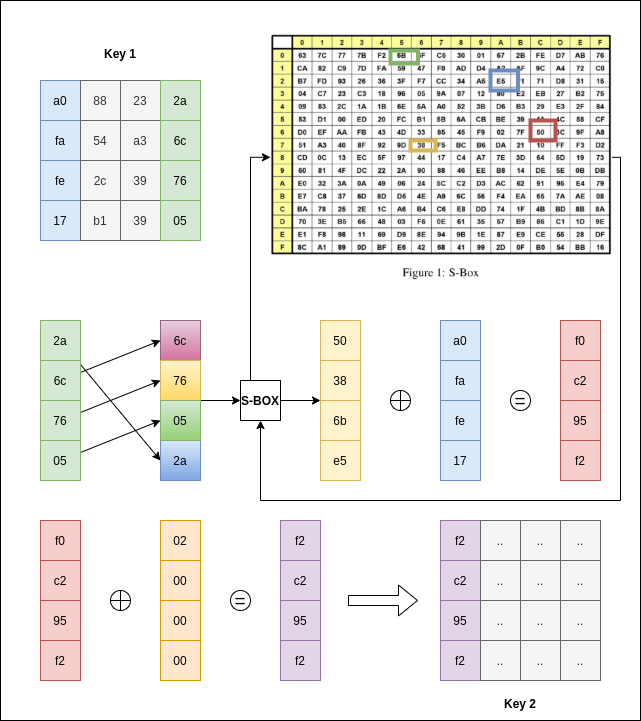
\includegraphics[width=300pt]{img/AESKey2.png}
 \caption{Calculating the first column of the second round key}
 \end{figure}




\newpage
\section{Q3}

ECB, CBC, OFB etc. are modes of operation in stream ciphers or when it comes to encrypting data that is longer than the block size given within a certain block cipher algorithm. For instance in AES, a block is 128 bits. If you however want to encrypt more data than this, we use for instance CBC in order to provide additional security across the blocks. The principle is to treat the blocks as a stream.

In this task we have been given these parameters for demonstrating the different modes of operation:
\begin{itemize}
\item{Plaintext: \textit{DCS-3101}}
\item{IV: \textit{NO}}
\item{Key: \textit{EU}}
\item{Block size: \textit{16 bits}}
\item{Encryption: \textit{XOR}}
\end{itemize}

The block size of sixteen bits means that each block will have two characters, and we will end up with four blocks.

Converted to binary, the plaintext string looks like this: 
\begin{tcolorbox}
\begin{center}
\textcolor{blue}{01000100 01000011 01010011 00101101 \\00110011 00110001 00110000 00110001}
\end{center}
\end{tcolorbox}

The block size of sixteen bits means that each block will have two characters, and we will end up with four blocks.

\begin{tcolorbox}
\begin{center}
\textcolor{blue}{
\makebox[1.5cm]{\textbf{DC}}:\qquad01000100 01000011\\
\makebox[1.5cm]{\textbf{S-}}:\qquad01010011 00101101\\
\makebox[1.5cm]{\textbf{31}}:\qquad00110011 00110001\\
\makebox[1.5cm]{\textbf{01}}:\qquad00110000 00110001}
\end{center}
\end{tcolorbox}

The key and IV converted to binary looks like this: 
\begin{tcolorbox}
\begin{center}
\textcolor{blue}{
\makebox[1.5cm]{\textbf{IV}}:\qquad01001110 01001111\\
\makebox[1.5cm]{\textbf{KEY}}:\qquad01000101 01010101}
\end{center}
\end{tcolorbox}



\newpage
\subsection{1. ECB}

\begin{figure}[H]
 \centering
  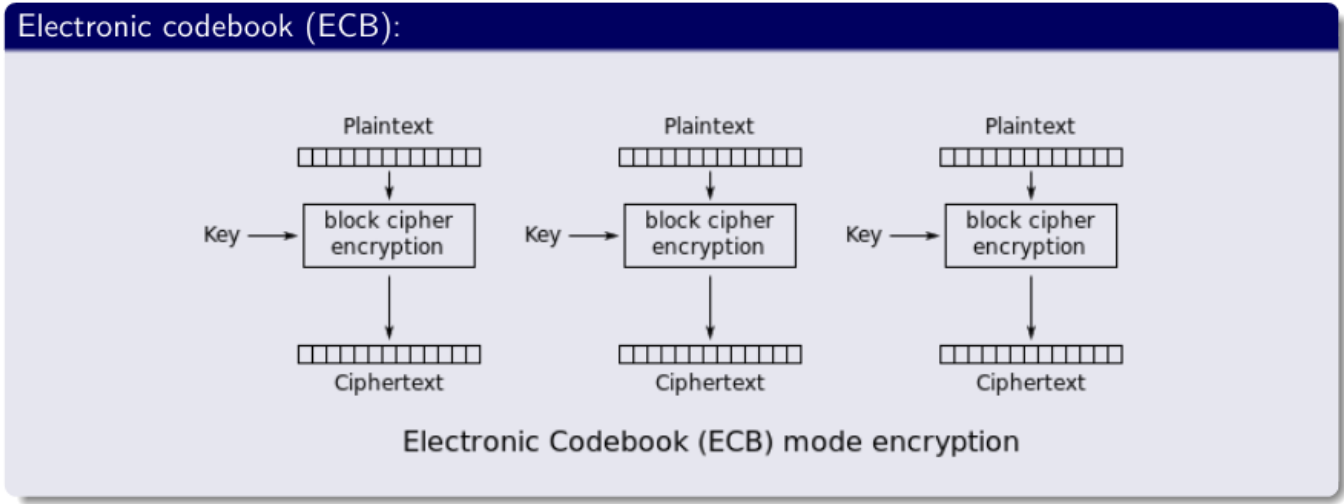
\includegraphics[width=300pt]{img/ecbLecture.png}
 \caption{ECB encryption diagram from lecture}
 \end{figure}


ECB is the simplest of the three modes of operation discussed in this assignment, and provide no additional security. The principle is to divide the text into blocks, encrypt them with whatever way we like, and concatenate the ciphertexts produced. This means that if you break one of the blocks, you will be able to break them all. However, an error will not propagate through the blocks. 

In practice it will look like this:
%%%FIX XOR FUNCTION

%DO THE REST IN HEX, THIS IS MADNESS!!!!
\begin{scriptsize}
\begin{tcolorbox}
\begin{center}
\textcolor{blue}{
 01000100 01000011\quad 01010011 00101101\quad  00110011 00110001\quad  00110000 00110001\\
\makebox[1.5cm]{\textbf{XOR}}\qquad  \makebox[1.5cm]{\textbf{XOR}}\qquad  \makebox[1.5cm]{\textbf{XOR}}\qquad  \makebox[1.5cm]{\textbf{XOR}}\\
01000101 01010101\quad 01000101 01010101\quad 01000101 01010101\quad 01000101 01010101\\
\makebox[1.5cm]{\textbf{=}}\\
00000001 00010110\quad 00010110 01111000\quad 01110110 01100100\quad 01110101 01100100
}

\end{center}
\end{tcolorbox}
\end{scriptsize}

\newpage
\subsection{2. CBC}

As the complexity grows in the following operation modes, we will from here on use hexadecimal numbers for increased readability.

In hex, the  input data, looks like this:
\begin{tcolorbox}
\begin{center}
\textcolor{blue}{
\makebox[1.5cm]{\textbf{DC}}:\qquad44 43\\
\makebox[1.5cm]{\textbf{S-}}:\qquad53 2d\\
\makebox[1.5cm]{\textbf{31}}:\qquad33 31\\
\makebox[1.5cm]{\textbf{01}}:\qquad30 31}
\end{center}
\end{tcolorbox}

The key and IV converted to binary looks like this: 
\begin{tcolorbox}
\begin{center}
\textcolor{blue}{
\makebox[1.5cm]{\textbf{IV}}:\qquad4e 4f\\
\makebox[1.5cm]{\textbf{KEY}}:\qquad45 55}
\end{center}
\end{tcolorbox}


\begin{figure}[H]
 \centering
  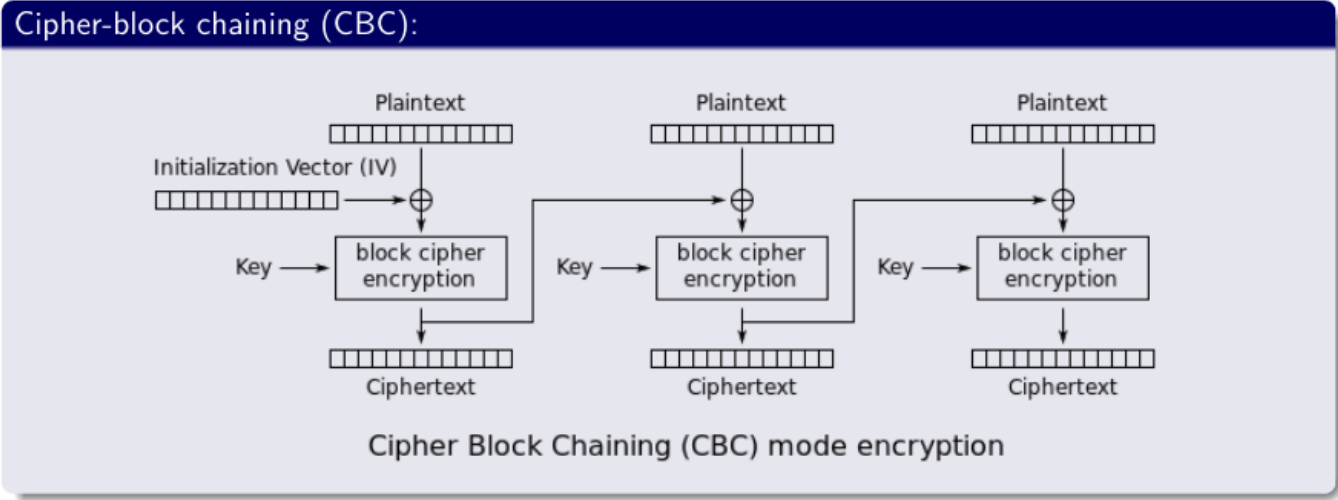
\includegraphics[width=300pt]{img/cbcLecture.png}
 \caption{CBC encryption diagram from lecture}
 \end{figure}

CBC stands for cipher-block chaining, and that is exactly what it does. Each plaintext block is XORed with the ciphertext of the previous block. For the first block, we XOR it with an IV (initialization vector). This ensures that each block is dependent on the previous one, and increases the security, as the breaking of one block, does not break the entire message. It does have error propagation however, so an error in a block, wil give an error in all the later blocks. 

In practice it looks like this: 
\begin{figure}[H]
 \centering
  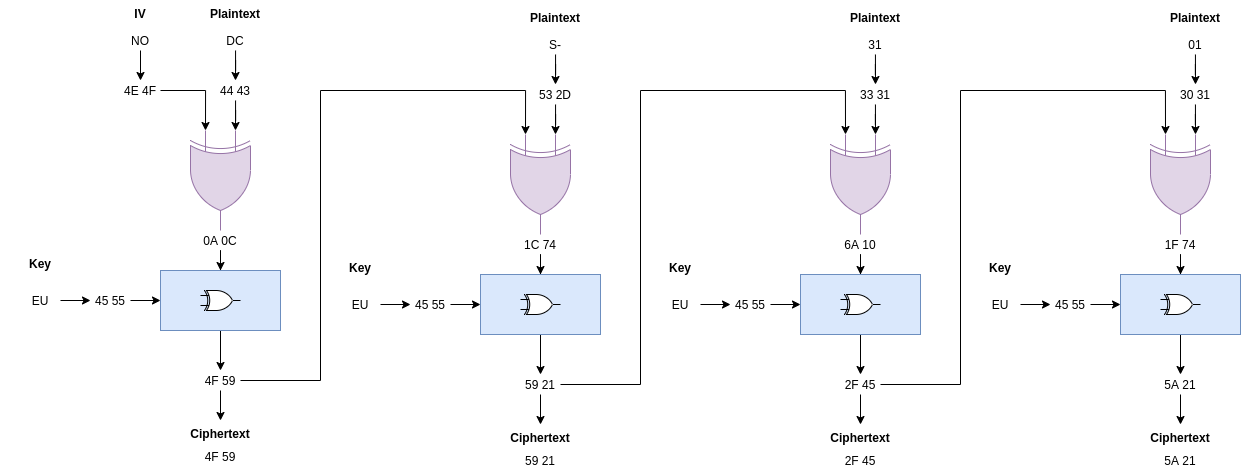
\includegraphics[width=400pt]{img/CBC.png}
 \caption{Illustration of CBC}
 \end{figure}

So the encrypted message becomes:
\begin{tcolorbox}
\begin{center}
\textcolor{blue}{
\makebox[1.5cm]{CBC Encrypted:}\qquad 4F 59 59 21 2F 45 5A 21}
\end{center}
\end{tcolorbox}





\newpage
\subsection{3. OFB}


\begin{figure}[H]
 \centering
  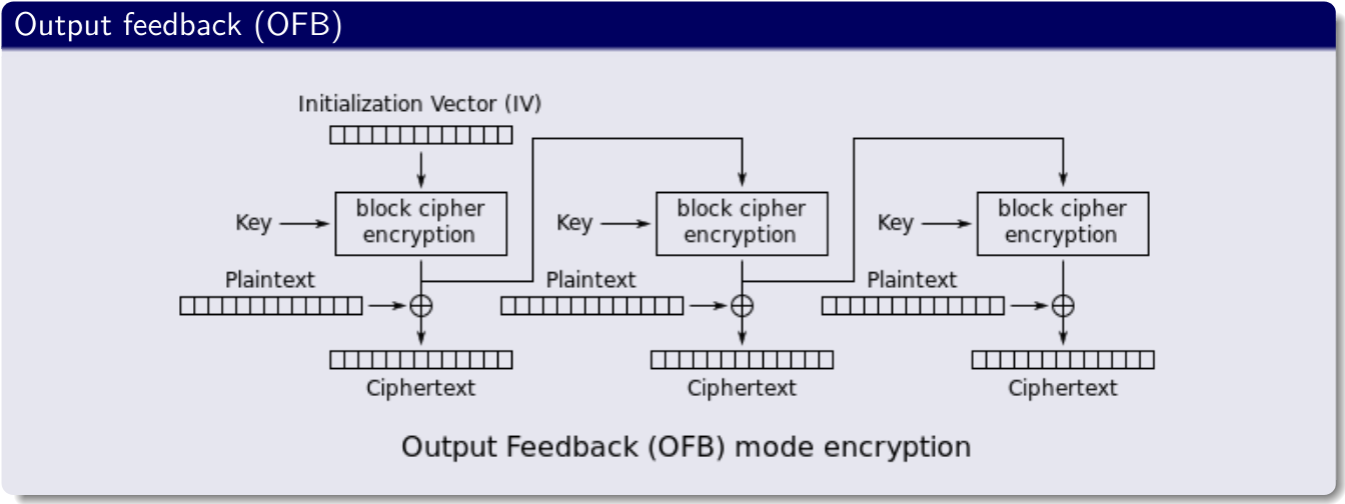
\includegraphics[width=300pt]{img/ofbEnLecture.png}
 \caption{OFB encryption diagram from lecture}
 \end{figure}

OFB (Output feedback), does the block encryption on the IV, rather than on the plaintext. It then XORS the plaintext with the output of the block encryption. The input in the following block encryptions however is the output of the previous block cipher (which does not involve the plaintext). Because of this no blocks are dependent on the plaintext or ciphertext of the previous block, which means that an error will only give an error in the current block (as we will see in the next part). 

In practice it looks like this:
\begin{figure}[H]
 \centering
  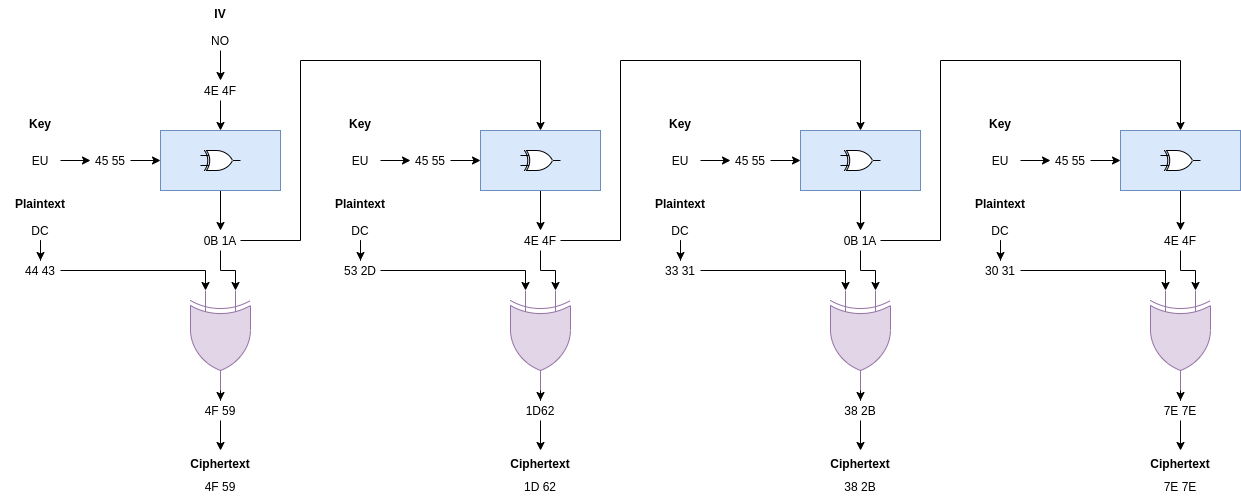
\includegraphics[width=400pt]{img/OFB.png}
 \caption{Illustration of OFB}
 \end{figure}

\begin{tcolorbox}
\begin{center}
\textcolor{blue}{
\makebox[1.5cm]{OFB Encrypted:}\qquad 4F 59 1D 62 38 2B 7E 7E}
\end{center}
\end{tcolorbox}


\newpage
\subsection{4. OFB - Decryption}

\begin{figure}[H]
 \centering
  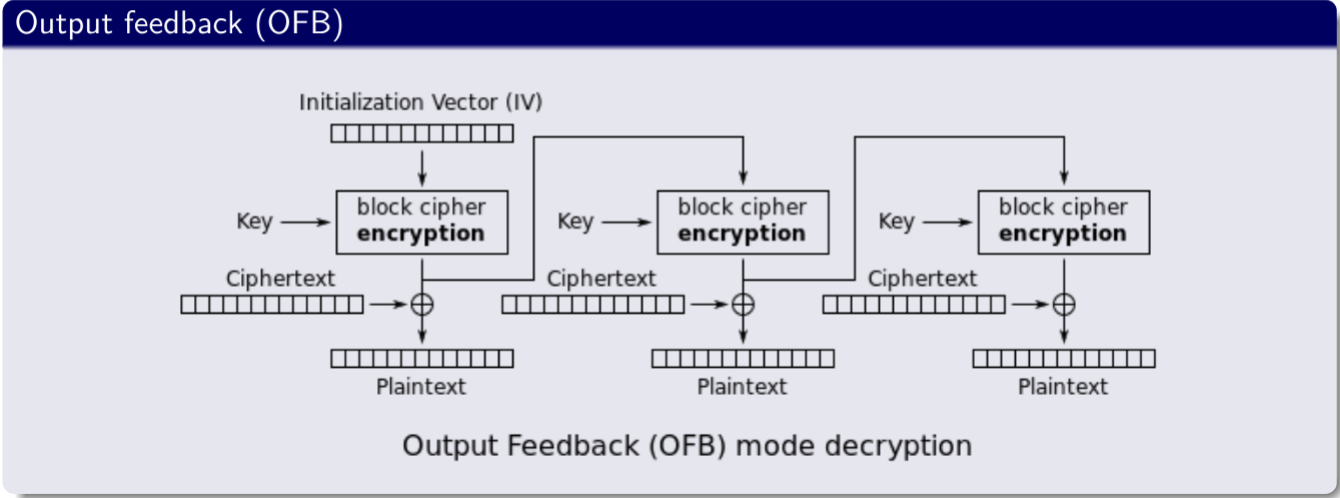
\includegraphics[width=300pt]{img/ofbDeLecture.png}
 \caption{OFB decryption diagram from lecture}
 \end{figure}

In this assignment we will flip the last bit of the first output of the first block from the previous task, and see the effect it has on the decrypted message. 

The ciphertext with the flipped bit, looks like this: 
\begin{tcolorbox}
\begin{center}
\textcolor{blue}{
\makebox[1.5cm]{Ciphertext: }\qquad 4F 58 1D 62 38 2B 7E 7E}
\end{center}
\end{tcolorbox}
The fourth hex digit 9, turned into an 8.


\begin{figure}[H]
 \centering
  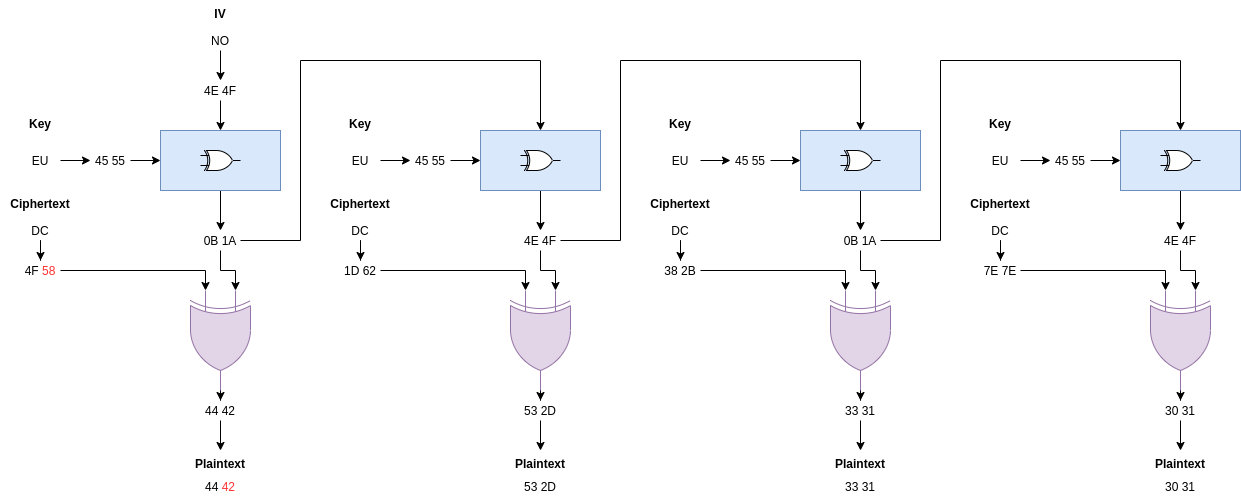
\includegraphics[width=400pt]{img/OFBDec.png}
 \caption{Illustration of OFB decryption with a flipped bit}
 \end{figure}

Decrypted message: 
\begin{tcolorbox}
\begin{center}
\textcolor{blue}{
\makebox[1.5cm]{Plaintext:}\qquad 44 42 53 2D 33 31 30 31}
\end{center}
\end{tcolorbox}


If we take the decrypted message and turn it back into text, it will look like this:
\begin{tcolorbox}
\begin{center}
\textcolor{blue}{
\makebox[1.5cm]{Plaintext:}\qquad DBS-3101}
\end{center}
\end{tcolorbox}

We can now see that the original C, has turned into a B. This corresponds with what we mentioned in the previous task, that the bit error only has an effect on one block. 

\subsection{Comparision}
If we compare the results from the three modes:
\begin{tcolorbox}
%\begin{center}
\textcolor{blue}{
\makebox[2cm]{ECB:}\qquad 01 16 16 78 76 64 75 64\\
\makebox[2cm]{CBC:}\qquad 4F 59 59 21 2F 45 5A 21\\
\makebox[2cm]{OFB:}\qquad 4F 59 1D 62 38 2B 7E 7E}
%\end{center}
\end{tcolorbox}

We of course see that they are drastically different. ECB is without the IV, so it will of course bear the least resemblance to the others. We can also see that while CBC and OFB start of similarly, they quickly diverge. 


\newpage
\section{Q4}

In cryptography it is common to separate between two different types of encryption, namely \textit{symmetric} and \textit{asymmetric}.

Symmetric encryption is the intuitive and oldest way of encrypting data, where one uses the same key to both encrypt and decrypt the data. There are countless examples of this, where perhaps the most common one today is AES. However the Caesar Cipher, Vignere Cipher and all encryption we did in task 3 are also examples of symmetric encryption. 

Asymmetric encryption (also known as public key cryptography), differs from this, as it uses different keys for encryption and decryption. If Alice encrypts a message, Bob will not be able to decrypt the message with the same key. He will have to have the sibling key in the key-pair, to be able to make sense of the encrypted message. The most common example of asymmetric encryption is RSA. 

In symmetric cryptography, we can usually in principle select any key we like. There are no inherent properties necessary within the key, so key generation is quite trivial. In asymmetric cryptography however, this is not the case. To generate an asymmetric key-pair, we use  mathematics to generate them. 

In the case of RSA, we use modulo arithmetic and large primes, and take advantage of the fact that it is difficult to factor two large primes multiplied together. 

The term public key cryptography comes with an interesting possibility that opens up when you have asymmetric encryption. Usually one takes the keys generated and refer to one of them as the public key, and the other as the private key. The public key you share openly while keeping the private key secret. 

The reason for doing this, is to let anyone encrypt data with the public key, whilst knowing that you will be the only one able to decrypt it. This is quite practical in and of itself, but in addition to this, if you encrypt data with your private key, anyone who unlocks it with your public key can be sure that the integrity of the message has not been compromised. 

These properties are not present in symmetric cryptography. Because of this, and the fact that the keys are generated with a lot more care, one usually argues that asymmetric cryptography is safer than symmetric cryptography. 

Still, symmetric cryptography has its place, as the complexity of asymmetric cryptography is much higher and requires more overhead. 

As I have understood it, a common approach is to use asymmetric cryptography, in order to agree on a symmetric key, and then do large data-transfers in the symmetric way. 


%Vedlegg
\section{Appendices}


\newpage
%Referanse
%\section{Referanser}

\nocite{*}
\bibliographystyle{plain}
\bibliography{ref}

\addcontentsline{toc}{section}{References}

\end{document}